\frame{\frametitle{Compound effect of alignment and illumination}
\renewcommand{\imagesizestring}{height}
\setlength{\imagesizea}{0.25\textheight}
\setlength{\imagesizeb}{0.15\textheight}
\setlength{\gapsizea}{-0mm}
\begin{tabular}[b]{cc@{}b{.5\textwidth}}
% Example for setting the heights of the images
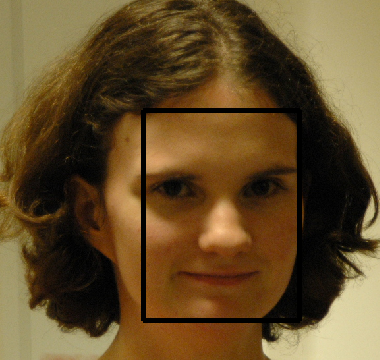
\includegraphics[\imagesizestring=\imagesizea]{figures_cvpr/promo/case1/detector.png}& \hspace{\gapsizea}
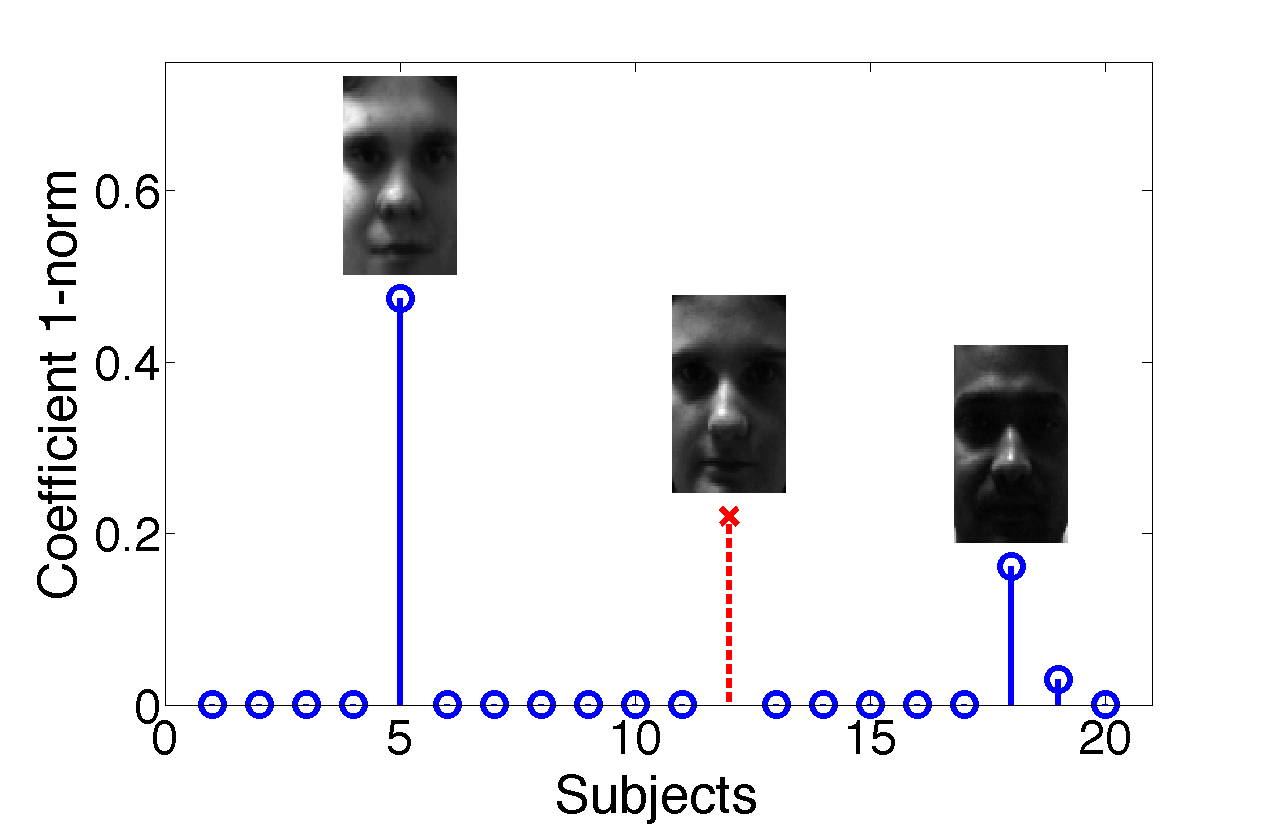
\includegraphics[\imagesizestring=\imagesizea]{figures_cvpr/promo/case1/sci_with_axis_face_case1.png} & 
{\bf Poor alignment}, Sufficient training illuminations \vfill\\
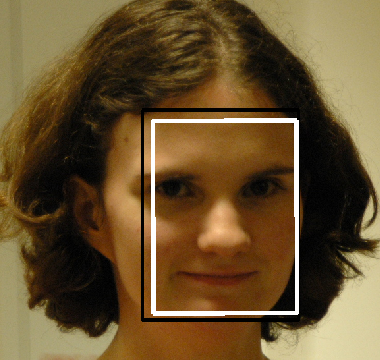
\includegraphics[\imagesizestring=\imagesizea]{figures_cvpr/promo/alignment_and_detector.png}& \hspace{\gapsizea}
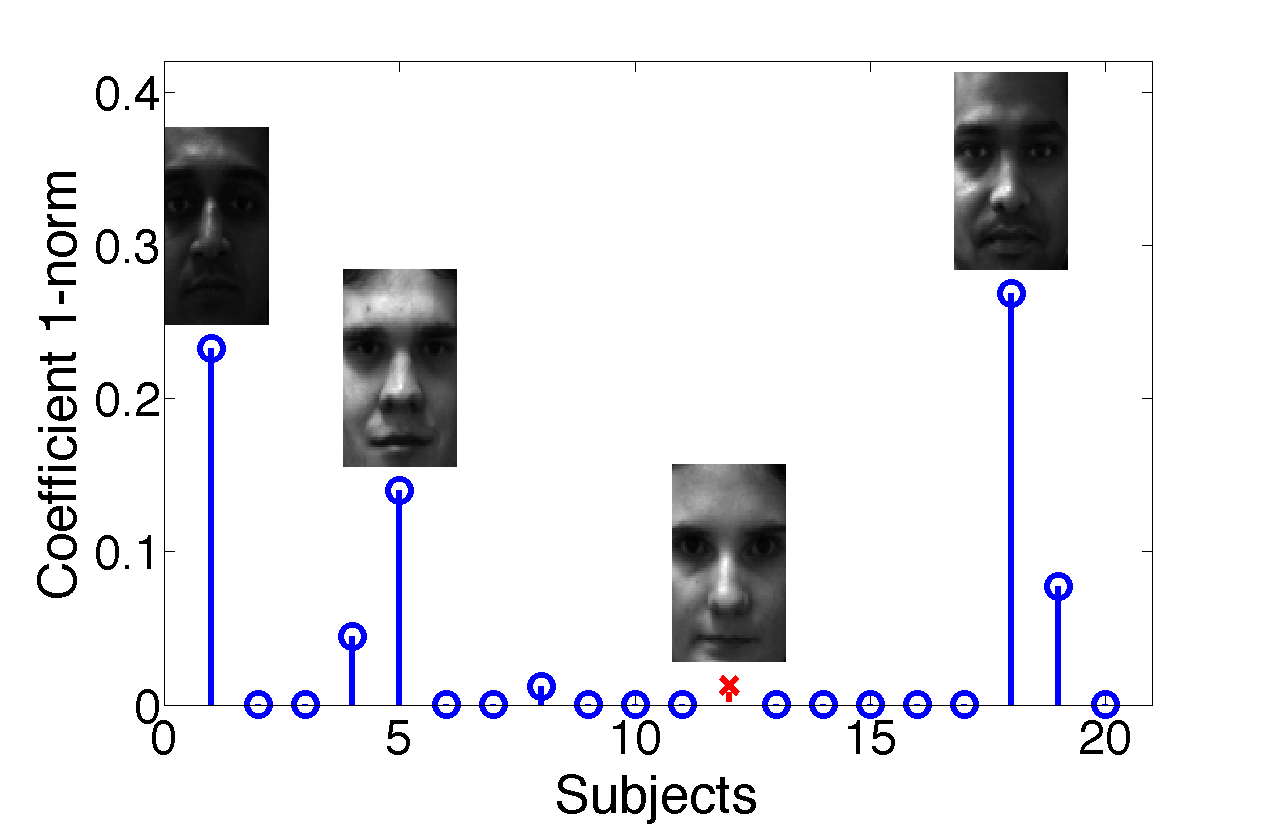
\includegraphics[\imagesizestring=\imagesizea]{figures_cvpr/promo/case2/sci_with_axis_face_case2.png} & 
{{\bf Good alignment}, Insufficient training illuminations}\vfill\\
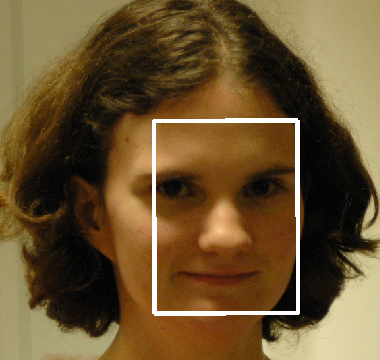
\includegraphics[\imagesizestring=\imagesizea]{figures_cvpr/promo/case3/alignment.png} & \hspace{\gapsizea}
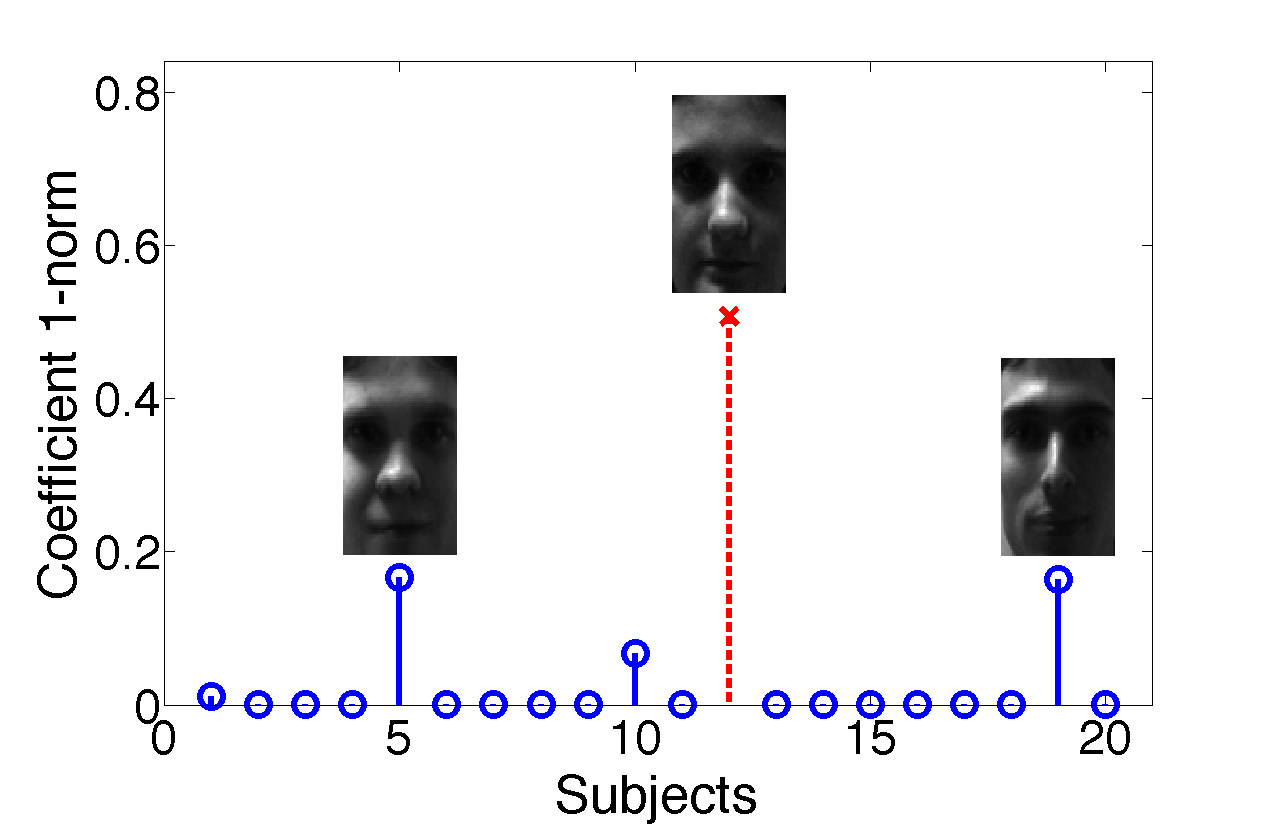
\includegraphics[\imagesizestring=\imagesizea]{figures_cvpr/promo/case3/sci_with_axis_face_case3.png} &
{{\bf Good alignment}, Sufficient training illuminations}\vfill
\end{tabular}
}
